\subsection{Inyectividad y Epiyectividad}
Una función $f(x)$ es \textit{inyectiva} cuando,
$\forall a,b \in X, \;\; f(a)=f(b) \Rightarrow a=b$
, es decir cuando nunca mapea elementos distintos de su \textit{Dominio} a un mismo elemento del \textit{Codominio}.

Análogamente, se dice que una función f(x) es \textit{sobreyectiva}, o epiyectiva cuando, $\forall y \in Y, \, \exists x \in X, \;\; f(x)=y$, es decir, que para cada elemento $y$ en el codominio $Y$, hay al menos un elemento $x$ en el dominio $X$ de forma que $f(x) = y$.\\
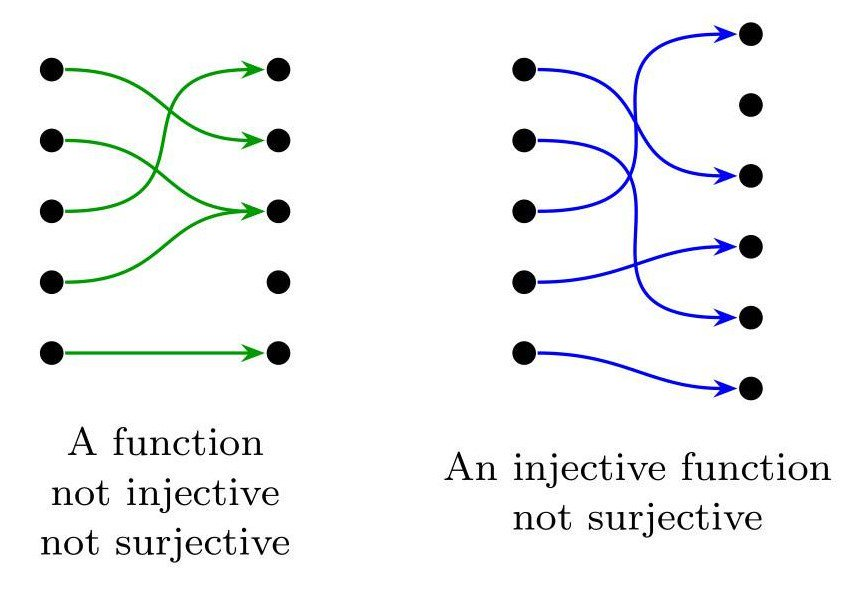
\includegraphics[width=\columnwidth]{inyectividad}\\
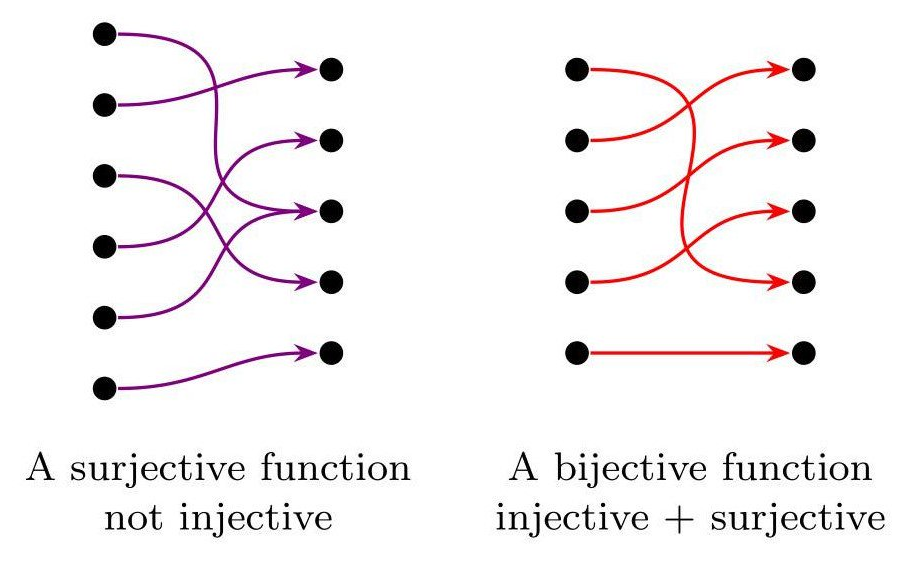
\includegraphics[width=\columnwidth]{sobreyectividad}
\subsection{Función Afín}
Una función afin tiene una \textbf{forma principal} de $y = mx + n$, donde se denomina lineal si $n=0$, y una \textbf{forma general} de $ax + by = 0$.\\
Para la forma general, $m = -\frac{a}{b}$ y $n = -\frac{c}{b}.$\\
Punto pendiente: $y - y_1 = m(x - x_1)$\\
Dos Puntos: $\frac{y-y_1}{x-x_1} = \frac{y_2-y_1}{x_2-x_1}$\\
Distancia punto-recta: $\frac{|ax_0+by_0+c|}{\sqrt{a^2+b^2}}.$\\
\textit{Nota:} $m = \tan \alpha$